
\documentclass{article}

%-------------------------------------------------------------------------------------------------------------
%  package
%--------------------------------------------------------------------------------------------------------------
%版面規劃(a4大小,上下左右距0.9inch)
\usepackage[a4paper,margin=0.9in]{geometry}
%作者資訊
\usepackage{authblk}
%中文化package
\usepackage{CJKutf8}

%分兩欄
\usepackage{multicol}
%分欄之後上圖需要有的package
\usepackage{float}
%然後若是需要在其中一欄上面加圖片=>[H大寫]
%要跨欄橫幅的圖片=>{figure*星號要加}[htbp]


%和插入圖片相關的package
\usepackage{graphicx}
\usepackage[tight]{subfigure}
\subfiguretopcaptrue
\usepackage{amsmath,booktabs,threeparttable,url, bm}
%\usepackage[hyphenbreaks]{breakurl}


%連結註腳網頁
\usepackage[colorlinks,linkcolor=blue]{hyperref}


%\newcommand{\cntext}{\begin{CJK}{UTF8}{bsmi}\end{CJK}}

\title{Assignment 9 of Computational Astrophysics in NTHU}
\author{Wei-Hsiang Yu 游惟翔}
\affil{Department of Physics, National Tsing Hua University, Hsinchu, Taiwan}

%-------------------------------------------------------------------------------------------------------------
%  文件開始
%--------------------------------------------------------------------------------------------------------------
\begin{document}

\begin{CJK}{UTF8}{bsmi}
%中文化需要加上此行才有title/author/date
\maketitle
\end{CJK}


%-------------------------------------------------------------------------------------------------------------
%  Written Assignments
%--------------------------------------------------------------------------------------------------------------
\section{Written Assignments}
\subsection*{Q1 : Estimate the mean free path $\lambda_{mfp}$ and collision time scale $\tau_{col}$}

Consider the neutral, atomic interstellar medium at $T=10^3$K.

On the Wikipedia\cite{b1} it provide the information of \textbf{cold neutral medium} \& \textbf{high neutral medium}

$$
\mbox{cold neutral medium  } (50-100K)
\mbox{     have \textbf{higher} density : }20-50
\ particle/cm^3
$$

$$
\mbox{high neutral medium  } (6000-10^{6}K)
\mbox{  have \textbf{lower} density : }0.2-0.5
\ particle/cm^3
$$

The interstellar medium we consider is in the interval between these two kinds of medium, so I suppose the density($particle/cm^3$) of neutral, atomic interstellar medium at $T=10^3$K is $n=1/cm^3$.

And the component of this interstellar medium is mainly hydrogen, so $\mu \sim 1m_{amu}$. The RMS speed $v \sim \sqrt{\frac{8kT}{\pi \mu}}=2.5 \times 10^5(cm/s)$
and the cross section $\sigma$ I use the value $\sigma \sim 3\times10^{-15} cm^2$ provided in lecture.


\begin{equation}
    \lambda_{mfp}\sim (n\sigma)^{-1} \sim 3.33\times10^{14}cm
    \label{eq:lambda}
\end{equation}

\begin{equation}
    \tau_{col}\sim (n\sigma v)^{-1} \sim 1.33\times10^{9}sec
    \label{eq:tau}
\end{equation}

\subsection*{Q2 : fluid approximation}
Consider a molecular cloud with:
$$
L=100pc=100\times(3.08\times10^{18})=3.08e20\mbox{ cm}
$$
$$
\tau=10^8yr=10^8\times(365\times86400)=3.1536e15\mbox{ sec}
$$

On the Wikipedia\cite{b1} it provide the information of molecular cloud :
$$
\mbox{molecular cloud  } (10-20K)
\mbox{     have density : }10^2-10^6
\ particle/cm^3
$$

if let $n=10^2$, $\lambda_{mfp}\sim 3.33\times10^{12}cm$; $\tau_{col}\sim 7.2\times10^{7}sec$.

\qquad $n=10^6$, $\lambda_{mfp}\sim 3.33\times10^{8}cm$; $\tau_{col}\sim 7.2\times10^{4}sec$.

Both length L and time $\tau$ scale is $>>$ than the mean free path $\lambda_{mfp}$ and collision time scale $\tau_{col}$, so we can viewed this molecular cloud as fluid.


\subsection*{Q3 : Conservation of momentum in hydrodynamic}
Derive\cite{b2}:

Given Euler equation:
\begin{equation}
    \frac{Dv}{Dt}=-\frac{\bigtriangledown P}{\rho}
    \label{eq:euler}
\end{equation}

By the convective derivate in the lecture and combine with Eq.\ref{eq:euler} we have:
\begin{equation}
    \frac{Dv}{Dt}
    \equiv \frac{\partial v }{\partial t}+(v \cdot \bigtriangledown)v
    =-\frac{\bigtriangledown P}{\rho}
    \label{eq:convective}
\end{equation}

By the continuity equation in the lecture we have:
\begin{equation}
    \frac{\partial \rho}{\partial t}=
    -(v \cdot \bigtriangledown)\rho-\rho(\bigtriangledown \cdot v)
    \label{eq:continuity}
\end{equation}

And we can make Eq.\ref{eq:convective} times $\rho$ and Eq.\ref{eq:continuity} times $v$, and add up to one equation.

\begin{equation}
    \rho \frac{\partial v }{\partial t}
    +v \frac{\partial \rho}{\partial t}
    =
    -\bigtriangledown P
    -\rho (v \cdot \bigtriangledown)v
    -v(v \cdot \bigtriangledown)\rho
    -\rho(\bigtriangledown \cdot v)v    
    \label{eq:combine}
\end{equation}

I recall the formula of gradient:
$$
    \bigtriangledown \cdot fA=f (\bigtriangledown \cdot A)+\bigtriangledown f \cdot A
$$

$$
\bigtriangledown \cdot (\rho v v)
=\rho \bigtriangledown \cdot (v v)+\bigtriangledown \rho \cdot (v v)
=\rho (v \cdot \bigtriangledown) v+\rho (v \cdot \bigtriangledown) v+\bigtriangledown \rho \cdot (v v)
$$

Using this $\bigtriangledown \cdot (\rho v v)$ term to substitute Eq.\ref{eq:combine}, we can finally get the form of Eq.\ref{eq:p_conservation}


\begin{equation}
    \frac{\partial \rho v}{\partial t}+\bigtriangledown \cdot (\rho v v +P \cdot I)=0
    \label{eq:p_conservation}
\end{equation}

%-------------------------------------------------------------------------------------------------------------
%  Programming Assignments
%--------------------------------------------------------------------------------------------------------------
\section{Programming Assignments}

%Q1---------------------------------------------------------------------
\subsection*{Q2 : Antares code for Kelvin-Helmholtz instability}
\subsubsection*{Q2.a}

\begin{equation}
    \mbox{initial condition : }
	\begin{cases}
	\rho=2,v_x=1,v_y=0, P=2.5, \mbox{\quad if } y>0.5\\
	\rho=1,v_x=-1,v_y=0, P=2.5, \mbox{ if } y<0.5
    \end{cases}
\end{equation}

I use momentum transform make $p=\rho \times v$ to get the momentum of each direction.

The energy can be gotten by two components: one is provided by inner energy u, can get by the equation of states(Eos) of pressure $P=(\gamma-1)u$;
the other is by kinetic energy $E_k$, $E_k=\frac{p^2}{2m}$.
(Show in Fig.\ref{fig:2khi_initial}.)

% %-------------------------------
\begin{figure}[h]
    \centering
    \subfigure[t=0]{
        
\includegraphics[scale=0.16]{t0.jpg}
        \label{fig:2_0_t0}
    }
    \subfigure[t=0.25]{
        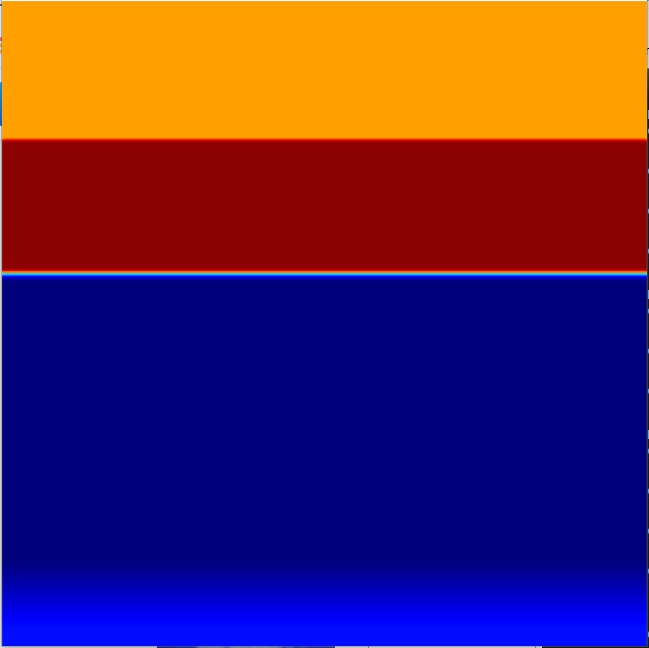
\includegraphics[scale=0.16]{t250.jpg}
        \label{fig:2_0_t25}
    }
    \subfigure[t=0.5]{
        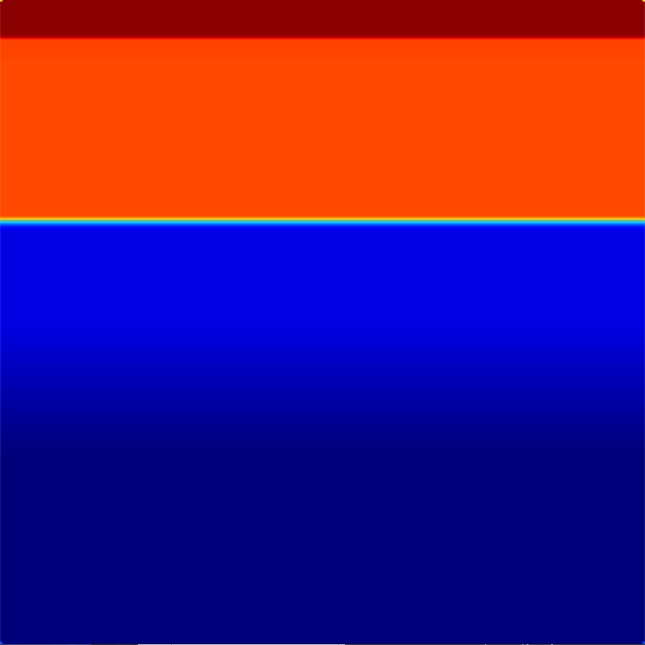
\includegraphics[scale=0.16]{t500.jpg}
        \label{fig:2_0_t50}
    }
    \subfigure[t=0.75]{
        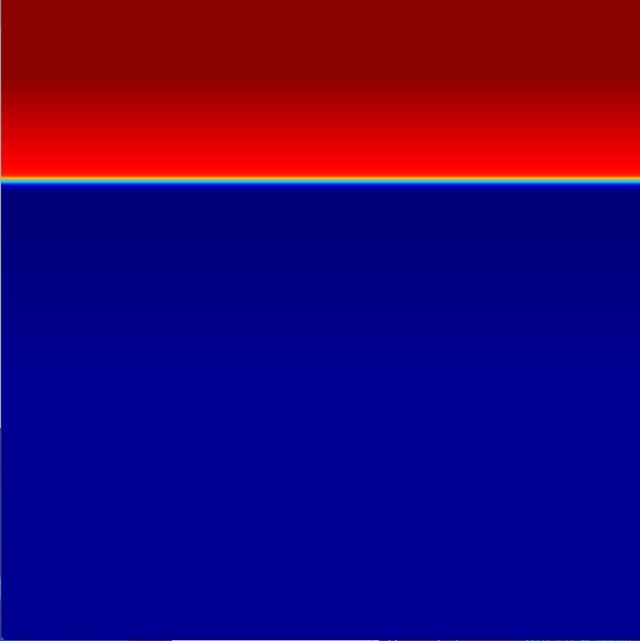
\includegraphics[scale=0.16]{t750.jpg}
        \label{fig:2_0_t75}
    }
    \subfigure[t=0.1]{
        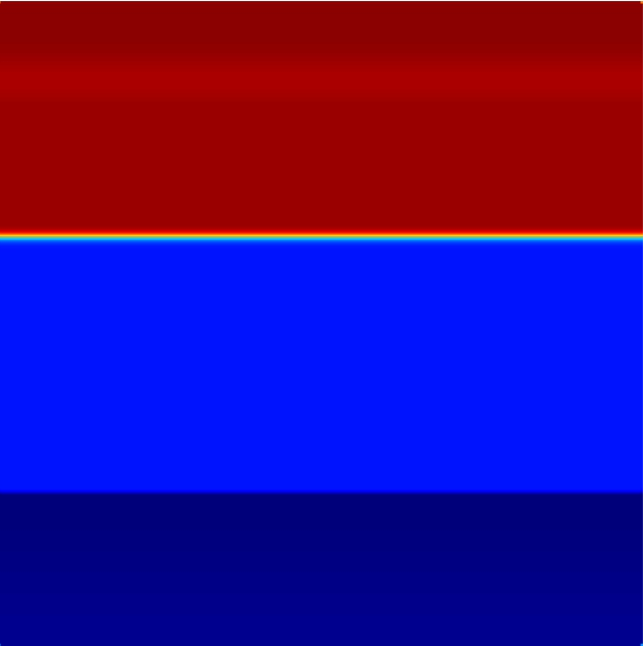
\includegraphics[scale=0.16]{t100.jpg}
        \label{fig:2_0_t1}
    }
    \caption{result of 2.a.}
    \label{fig:2_0}
\end{figure}
% %-------------------------------

\subsubsection*{Q2.b}
In this part, although I don't get the phenomenon of Kelvin-Helmholtz instability cloud like the question show, but change the boundary condition of this problem will get cool result.
In Fig.\ref{fig:2_1}, I make x direction has reflect boundary and y direction has periodic boundary, the contrary condition compare to origin(Fig.\ref{fig:2_0})
% %-------------------------------
\begin{figure}[h]
    \centering
    \subfigure[t=0]{
        
\includegraphics[scale=0.16]{t0.jpg}
        \label{fig:2_1_t0}
    }
    \subfigure[t=0.25]{
        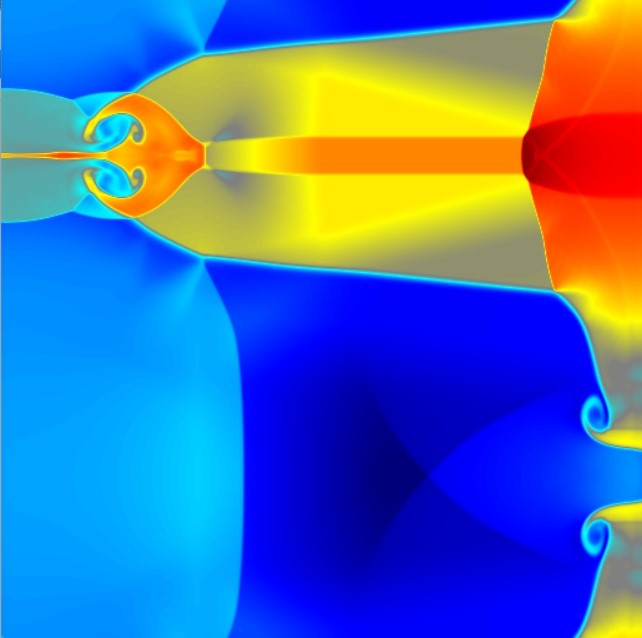
\includegraphics[scale=0.16]{t251.jpg}
        \label{fig:2_1_t25}
    }
    \subfigure[t=0.5]{
        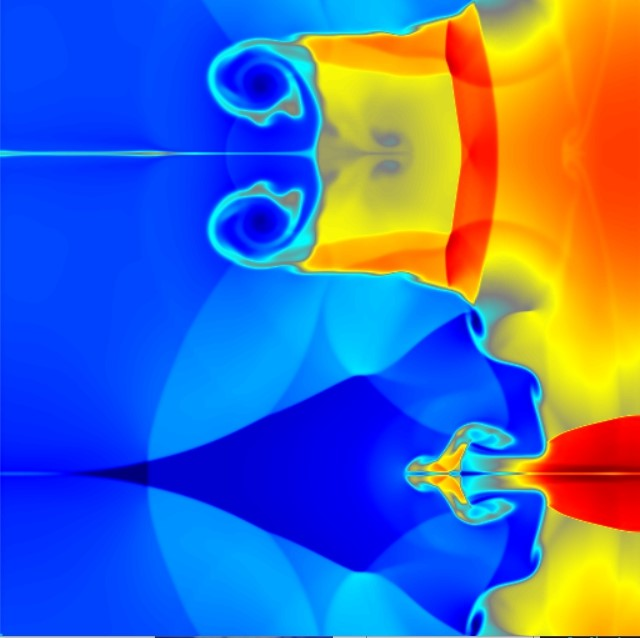
\includegraphics[scale=0.16]{t501.jpg}
        \label{fig:2_1_t50}
    }
    \subfigure[t=0.75]{
        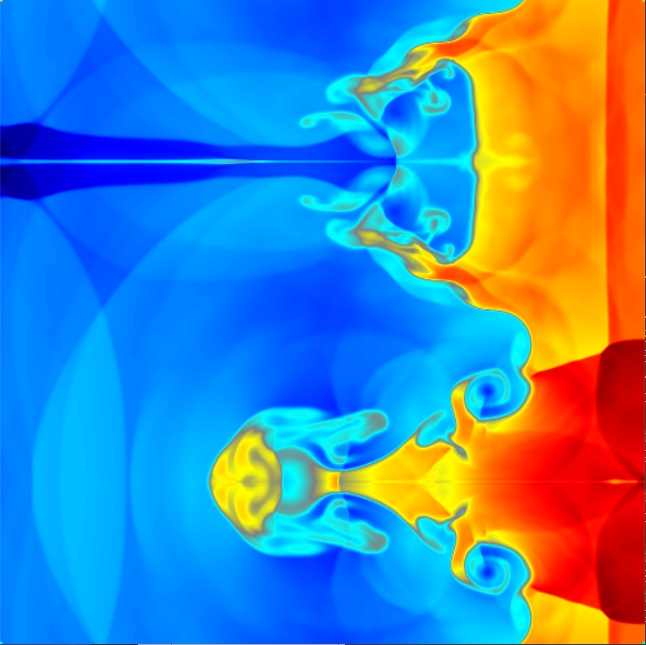
\includegraphics[scale=0.16]{t751.jpg}
        \label{fig:2_1_t75}
    }
    \subfigure[t=0.1]{
        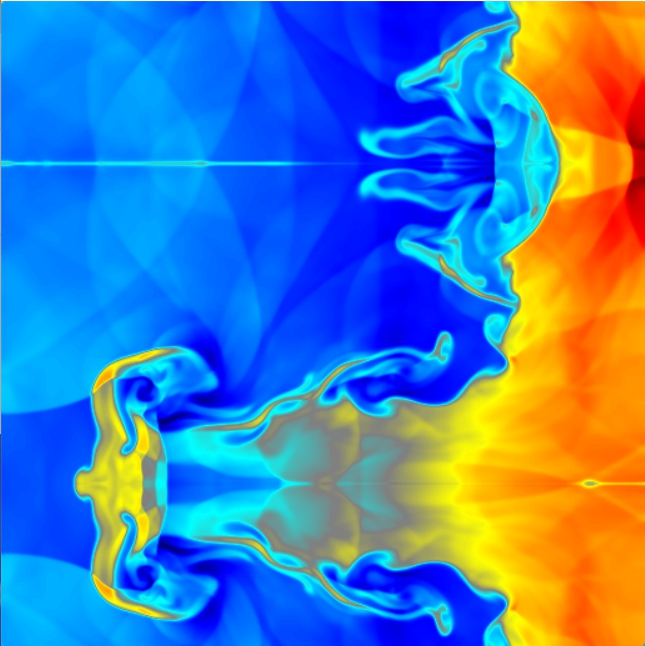
\includegraphics[scale=0.16]{t101.jpg}
        \label{fig:2_1_t1}
    }
    \caption{result of change the boundary condition}
    \label{fig:2_1}
\end{figure}
% %-------------------------------

% %-------------------------------
\begin{figure}[h]
    \centering
    \subfigure[initial condition]{
        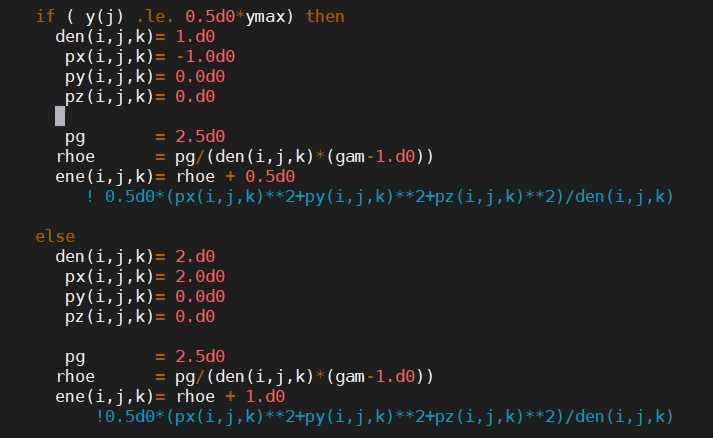
\includegraphics[scale=0.43]{initial.jpg}
        \label{fig:2khi_initial}
    }
    \subfigure[boundary condition]{
        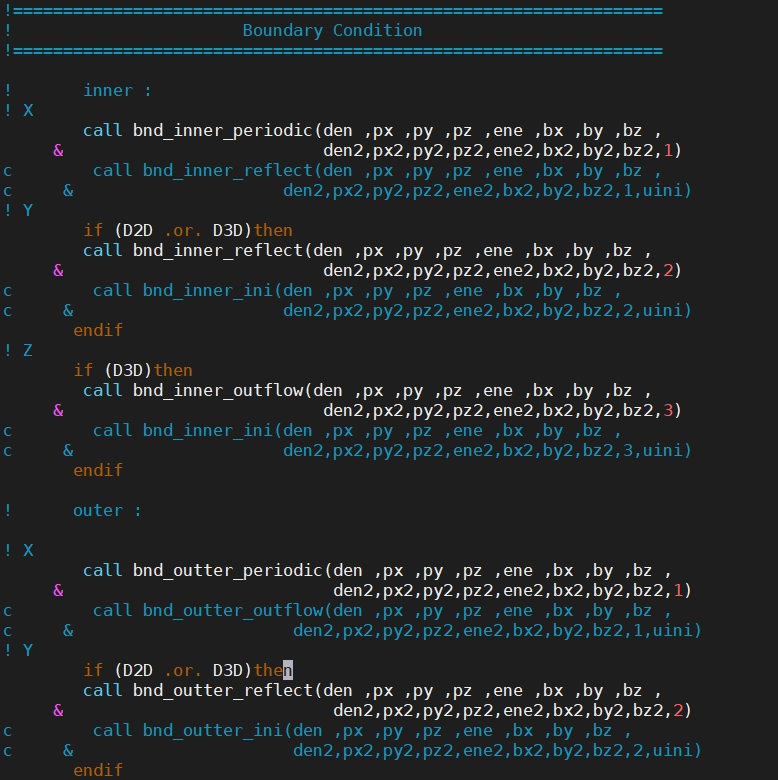
\includegraphics[scale=0.45]{boundary.jpg}
        \label{fig:2khi_boundary} 
    }
    \subfigure[parameter]{
        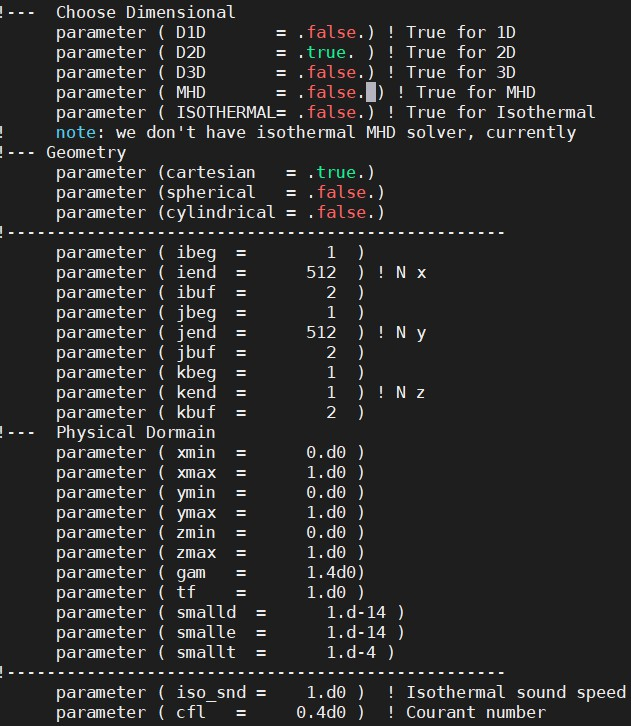
\includegraphics[scale=0.43]{parameter.jpg}
        \label{fig:2khi_parameter} 
    }
    \caption{problem set of folder \textbf{khi}}
    \label{fig:2khi}
\end{figure}
% %-------------------------------




\begin{thebibliography}{00}

\bibitem{b1}
Interstellar medium on Wikipedia\\
 \href{https://en.wikipedia.org/wiki/Interstellar\_medium}{https://en.wikipedia.org/wiki/Interstellar\_medium}
 
\bibitem{b2}
Conservation of momentum in hydrodynamic \\
\href{https://slidetodoc.com/lecture-planet-formation-topic-introduction-to-hydrodynamics-and/}{https://slidetodoc.com/lecture-planet-formation-topic-introduction-to-hydrodynamics-and\_/}

\end{thebibliography}

\end{document}

% \footnote{Lagrangian point:\href{https://en.wikipedia.org/wiki/Lagrange\_point}{https://en.wikipedia.org/wiki/Lagrange\_point}}


% %-------------------------------
% \begin{figure}[h]
%     \centering 
% 	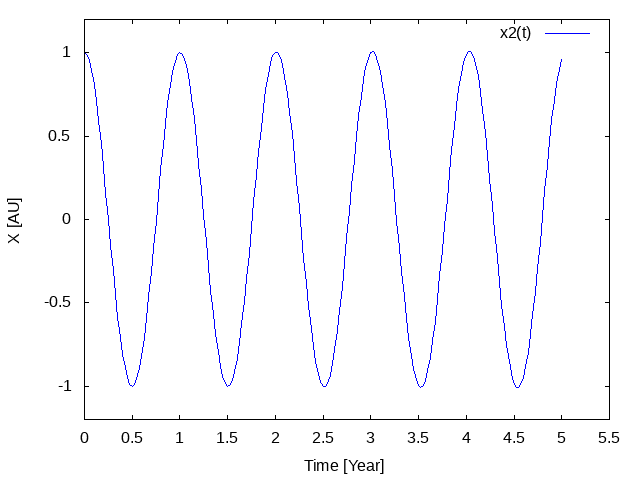
\includegraphics[scale=0.45]{pro1_x2.png}
% 	\caption{The trajectory of $m_1$ $m_2$ (when $m_2$ has a 1.25 factor of velocity).} %圖片註解
% 	\label{fig.pro1} %label 用這個就可以引用文章當中
% \end{figure}
% %-------------------------------

% %-------------------------------
% \begin{figure}[h]
%     \centering
%     \subfigure[dt=0.01yr]{
%         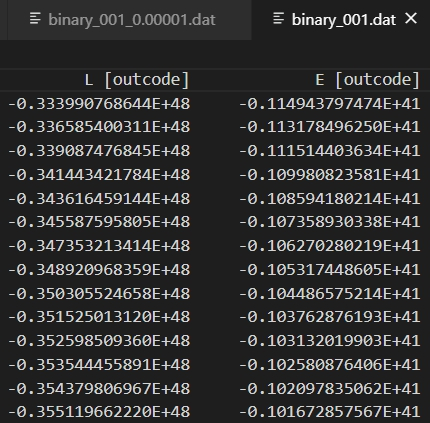
\includegraphics[scale=0.33]{01.jpg}
%         \label{01}
%     }
%     \subfigure[dt=0.001yr]{
%         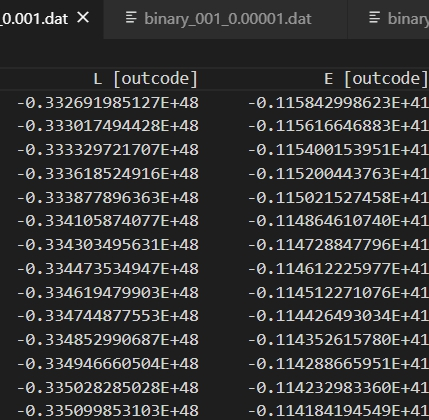
\includegraphics[scale=0.33]{001.jpg}
%         \label{001} 
%     }
%     \subfigure[dt=0.00001yr]{
%         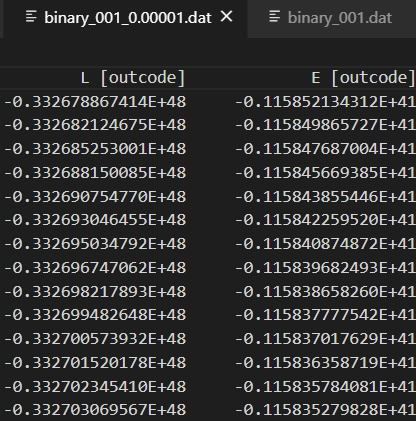
\includegraphics[scale=0.33]{00001.jpg}
%         \label{00001} 
%     }
%     \caption{L \& E in 0.01,0.001,0.00001 time step}
%     \label{fig:2c_dat}
% \end{figure}
% %-------------------------------